\section{Задание №3}

\begin{enumerate}
        \item Построить датчик экспоненциального распределения. 
        Проверить для данного распределения свойство отсутствия памяти. Пусть $X_1,\,X_2,\,\ldots,\,X_n$ независимо распределенные случайные величины с параметрами $\lambda_1,\,\lambda_2,\,\ldots,\,\lambda_n$ соответственно. 
        Найти распределение случайной величины $Y = \min\{\,X_1,\,X_2,\,\ldots,\,X_n\,\}$.
        \item На основе датчика экспоненциального распределения построить датчик пуассоновского распределения.
        \item Построить датчик пуассоновского распределения как предел биномеального распределения.
        С помощью критерия хи-квадрат Пирсона убедиться, что получен датчик распределения Пуассона.
        \item Построить датчик стандартного распределения методом моделирования случайных величин парами с переходом в полярные координаты. Проверить при помощи t-критерия Стьюдента равенство математических ожиданий, а при помощи критерия Фишера --- равенство дисперсий.
\end{enumerate}


\subsection{Построение датчика экспоненциальной случайной величины}

\begin{definition}
        Будем говорить, что случайная величина $X$ \textit{имеет экспоненциальное распределение с параметром $\lambda > 0$}, если ее функция распределения имеет вид
$$
        F_X(x) = 
        \begin{cases}
                1 - e^{-\lambda x},& \mbox{при $x \geqslant 0$,} \\
                0, & \mbox{при $x < 0$.}
        \end{cases}
$$
        Будем обозначать такие случайные величины
$$
        X \sim \mbox{Exp}(\lambda).
$$
\end{definition}

Для того чтобы построить датчик экспоненциально распределенной с параметром $\lambda$ случайной величины $X$, воспользуемся методом обратной функции распределения (смотри теорему~\ref{th:inv-method}). Получается, что такую случайную величину можно представить в виде:
$$
        X =
        F_x^{-1}(\xi) =
        -\frac{1}{\lambda}\ln(1 - \xi),
$$
где $\xi$~--- равномерно распределенная на отрезке $[0,\,1]$ случайная величина.


\subsection{Отсутствие памяти у экспоненциального распределения}

\begin{assertion}[Свойство отсутствия памяти]
        Пусть $X\sim\mbox{Exp\,}(\lambda)$, тогда для любых $t \neq 0$ и $s$ справедливо:
$$
        \p(X\geqslant s+t\,|\,X\geqslant t) =
        \p(X \geqslant s).
$$
\end{assertion}

\begin{proof}
        Рассмотрим левую часть равенства:
$$
        \p(X \geqslant s + t\,|\,X\geqslant t) =
        \frac{\p(X \geqslant s + t,\,X\geqslant t)}{\p(X\geqslant t)} =
        \frac{\p(X \geqslant s + t)}{\p(X\geqslant t)}.
$$
Таким образом получаем, утверждение эквивалентно тому, что
$$
        \p(X\geqslant s+t) = 
        \p(X\geqslant t)\p(X\geqslant s).
$$
Из определения функции распределения $F_X(t) = \p(X < t) = 1 - \p(X \geqslant t)$ получаем, что
$$
        e^{-\lambda(s+t)} = e^{-\lambda s}e^{-\lambda t}.
$$
Последнее равенство точно верно. Таким образом, утверждение доказано.
\end{proof}


\subsection{Распределение минимума экспоненциальных случайных величин}

Рассмотрим теперь случайную величину $Y = \min\{\,X_1,\,X_2,\,\ldots,\,X_n\,\}$, где $X_i, i = \overline{1,\,n}$ есть независимо распределенные экспоненциальные случайные величины с параметрами $\lambda_1,\,\lambda_2,\,\ldots,\,\lambda_n$ соответственно, и найдем её функцию распределения:
\begin{multline*}
        F_Y(x) =
        \p(Y < x) = 
        \p (\min\limits_{i = \overline{1,\,n}} X_i < x) =
        1 - \p (\min\limits_{i = \overline{1,\,n}} X_i \geqslant x) =
        \\
        = 1 - \p(X_1 \geqslant x,\,X_2 \geqslant x,\,\ldots,\,X_n \geqslant x) =
        1 - \prod_{i = 1}^{n} \p (X_i \geqslant x) = 
        1 - \prod_{i = 1}^n(1 - F_{X_i}(x)).
\end{multline*}
Таким образом функция распределения случайной величины $Y$ представима в виде
$$
        F_Y(x) = 1 - \prod_{i = 1}^n (1 - 1 + e^{\lambda_i x}) =
        1 - \prod_{i = 1}^n e^{\lambda_i x} = 1 - e^{(\lambda_1 + \lambda_2 + \ldots + \lambda_n)x}.
$$
Получается, что заданная случайная величина $Y$ имеет экспоненциальное распределение с параметром $\lambda = \lambda_1 + \lambda_2 + \ldots + \lambda_n$.


\subsection{Построение датчика распределения Пуассона}

\begin{definition}
        Будем говорить, что случайная величина $X$ \textit{имеет распределение Пуассона с параметром $\lambda > 0$}, если
$$
        \p(X = k) = \frac{\lambda^k}{k!} e^{-\lambda},
        \quad
        \mbox{где } k \in \N_0.
$$
Будем обозначать такие случайные величины
$$
        X \sim \mbox{Pois}(\lambda).
$$
\end{definition}

Для построения датчика Пуассоновской случайной величины докажем вспомогательное утверждение.
\begin{assertion}[О распределении суммы экспоненциальных случайных величин]
\label{th:2-2-1}
        Пусть $S_n = \sum_{i=1}^n \xi_i$, где $\xi_i\sim\mbox{Exp}(\lambda)$, $i = \overline{1,\,n}$.
        Тогда
$$
        F_{S_n}(x) = 1 - e^{-\lambda x}\sum_{k = 0}^{n-1} \frac{\lambda^k x^k}{k!}.
$$
\end{assertion}
\begin{proof}
        Для доказательства достаточно показать, что случайная величина~$S_n$ имеет плотность распределения, равную
$$
        \rho_{S_n}(x) = e^{-\lambda x}\frac{\lambda^{n}x^{n-1}}{(n-1)!},\quad x\geqslant 0.
$$
Докажем это методом математической индукции.
База индукции очевидна.
Теперь пусть для шага $n$ выполнена предыдущая формула.
Воспользуемся формулой свертки плотностей распределений для нахождения $\rho_{S_{n+1}}$
$$
        \rho_{S_{n+1}}(x)
        =
        \int_0^x \rho_{S_1}(x - t)\cdot\rho_{S_n}(t)\,dt
        =
        \frac{\lambda^{n+1}}{(n-1)!}e^{-\lambda x}\int_0^x (x-t)^{n-1}\,dt
        =
        \frac{\lambda^{n+1}}{(n-1)!} e^{-\lambda x}\frac{x^n}{n}.
$$
Теорема доказана.

\end{proof}

Пусть $t > 0$. Рассмотрим независимые случайные величины $\{\xi_k\}_{k \geqslant 1}$, имеющие показательное распределение с параметром $\lambda$. Как и в предыдущем утверждении, положим $S_n = \sum_{k=1}^n \xi_k$. Наконец, обозначим $X = \max\{\,n\geqslant 0\;|\;S_n < t\}$, полагая $S_0 = 0$. Докажем теперь, что $X\sim\mbox{Pois}(\lambda t)$.

Для этого найдем вероятность того, что $X = n$. При $n = 0$
$$
        \p (X = n) = \p (\xi_1 \geqslant t) = e^{\lambda t}.
$$
При $n > 0$, поскольку $\xi_k \geqslant 0$, то согласно утверждению~\ref{th:2-2-1}
\begin{multline*}
        \p (X = n) 
        =
        \p (S_n < t,\, S_{n+1} \geqslant t)
        =
        \p(S_n < t) - \p(S_n < t,\,S_{n+1} < t)
        = \\ =
        \p(S_n < t) - \p(S_{n+1} < t)
        =
        F_{S_n}(t) - F_{S_{n-1}}(t)
        =
        \frac{\lambda^n t^n}{n!}e^{-\lambda t}.
\end{multline*}

Таким образом мы получали способ построения пуассоновской случайной величины. Нужно просто брать показательные случайные величины с параметром $\lambda = 1$ и смотреть сумма скольки первых из них меньше параметра пуассоновского распределения.


\subsection{Построение датчика распределения Пуассона как предел биномиального распределения}

Биномиальное распределение сходится к распределению Пуассона, так как число испытаний уходит в бесконечность, в то время как произведение $np$ остается фиксированным или, по крайней мере, $p$ стремится к нулю. Поэтому распределение Пуассона с параметром $\lambda = np$ можно использовать как приближение к $\mbox{Bin }(n,\,p)$ биномиального распределения, если $n$ достаточно велико, а $p$ достаточно мало. Подробное доказательство этого факта, а также эмперические правила выбора параметров биномиального распределения и оценки точности приближения можно посмотреть в \cite{counts_control_charts} и \cite{novak}[Глава~4]. Мы же попытаемся лишь обосновать сам факт этого.

Пусть случайная величина $\xi$ имеет биномиальное распределение с параметрами $n$ и $p$. И введем обозначение:
$$
        \p_n(\xi = k)
        =
        C_n^k p^k (1 - p)^{n-k}.
$$
Зафиксируем значение $\lambda = np$, которое является математическим ожиданием биномиального распределения и будем устремлять параметр $n$ к бесконечности:
\begin{multline*}
        \lim_{n\to\infty}\p_n(k)
        =
        \lim_{n\to\infty}\left[C_n^k\cdot \left(\frac{\lambda}{n}\right)^k\cdot\left(1 - \frac\lambda n \right)^{n-k}\right]
        =\\=
        \frac{\lambda^k}{k!} \cdot e^{-\lambda} \cdot \lim_{n\to\infty}\left[ \frac{n!}{n^k(n-k)!} \left( 1 - \frac\lambda n \right)^{-k} \right]
        = \\ =
        \frac{\lambda^k}{k!} \cdot e^{-\lambda} \cdot \lim_{n\to\infty}\left[ \frac{n(n-1)\ldots(n-k+1)}{n^k} \left( 1 - \frac\lambda n \right)^{-k} \right]
        =
        \frac{\lambda^k}{k!} e^{-\lambda}.
\end{multline*}

\subsection{Проверка корректности работы датчика}

Для проверки правильности работы датчика пуассоновской случайной величины воспользуемся \textit{критерием согласия Пирсона} (или критерием согласия $\chi$-квадрат). Это один из наиболее популярных критериев для проверки гипотезы о принадлежности наблюдаемой выборки  некорому теоретическому закону распределения.

\begin{theorem}[Критерий согласия Пирсона]
        Обозначим нулевую гипотезу $H_0$ как гипотезу о том, что выборка $\xi_1,\,\xi_2\,\ldots\xi_n$ подчиняется закону распределения $\p$. Обозначим за $n_k$ количество элементов в выборке, равных $k$. За $r$ обозначим количество различных элементов выборки. А за $p_k$ --- вероятность выпадения значения в теоретическом распределении $p_k = \p(\xi = k)$. Введем статистику критерия
$$
        X^2_n = n \sum_{k = 1}^r
        \frac{\left(\frac{n_k}{n} - p_k\right)^2}{p_k}.
$$
        Тогда если гипотеза $H_0$ верна, то при увеличении $n$ статистика $X^2_n$ стремится к распределению $\chi^2$ c $r-1$ степенью свободы.
\end{theorem}

\begin{remark}
        Функция распределения $\chi^2$ c $l$ степеней свододы выглядит следующим образом:
$$
        F_{\chi^2_l} = 
        \frac
        {\gamma(\nicefrac{l}{2},\,\nicefrac{x}{2})}
        {\Gamma(\nicefrac{l}{2})},
        \quad
        \mbox{где } \Gamma \mbox{ и } \gamma \mbox{ обозначают полную и неполную гамма-функции.}
$$
        Такое определение делает почти невозможным аналитический поиск квантилей этой функции распределения. По этой причине для данных расчетов мы будем пользоваться встроенной в систему \texttt{Matlab} функцией \texttt{chi2inv(l, alpha)}, которая возвращает квантиль $\chi^2$-распределения c \texttt{l} степенями свободы порядка \texttt{alpha}.  
\end{remark}
\subsection{Задача №4}
\begin{definition}
        \texttt{Нормалное распределение --- это ...}
\end{definition}

Рассмотрим случайную величину $Z = \sqrt{2\xi}\sin\eta$, где $\xi\sim\mbox{Exp}\,(1)$, $\eta\sim\mbox{U}[0,2\,\pi] \sim 2\pi\mbox{U}[0,\,1]$. Тогда
\begin{multline*}
        \p(Z < x)
        =
        \p(\sqrt{2\xi}\sin\eta < x)
        =
        \iint\limits_{\{\,(\xi,\,\eta)\,|\,\sqrt{2\xi}\sin\eta<x\,\}} \frac{e^{-\xi}}{2\pi}\,d\xi d\eta
        =
        \left\{\,\xi = \frac{\psi^2}{2}\,\right\}
        = \\ =
        \iint\limits_{\{\,(\psi,\,\eta)\,|\,\psi\sin\eta<x\,\}} \frac{e^{-\frac{\psi^2}{2}}}{2\pi}\psi\,d\psi d\eta
        =
        \{\,X = \psi\cos\eta,\,Y = \psi\sin\eta\,\}
        = \\ =
        \iint\limits_{\{\,(X,\,Y)\,|\,Y < x\,\}} \frac{e^{-\frac{X^2}{2}}e^{-\frac{Y^2}{2}}}{2\pi}\,dXdY
        =
        \int\limits_{-\infty}^{+\infty}\frac{e^{-\frac{X^2}{2}}}{\sqrt{2\pi}}\,dX \int\limits_{-\infty}^{x} \frac{e^{-\frac{Y^2}{2}}}{\sqrt{2\pi}}\,dY
        =
        \int\limits_{-\infty}^{x}\frac{e^{-\frac{Y^2}{2}}}{\sqrt{2\pi}}\,dy.
\end{multline*}
Таким образом случайная величина $Z$ имеет стандартное нормальное распределение.
\clearpage
\begin{figure}[t]
        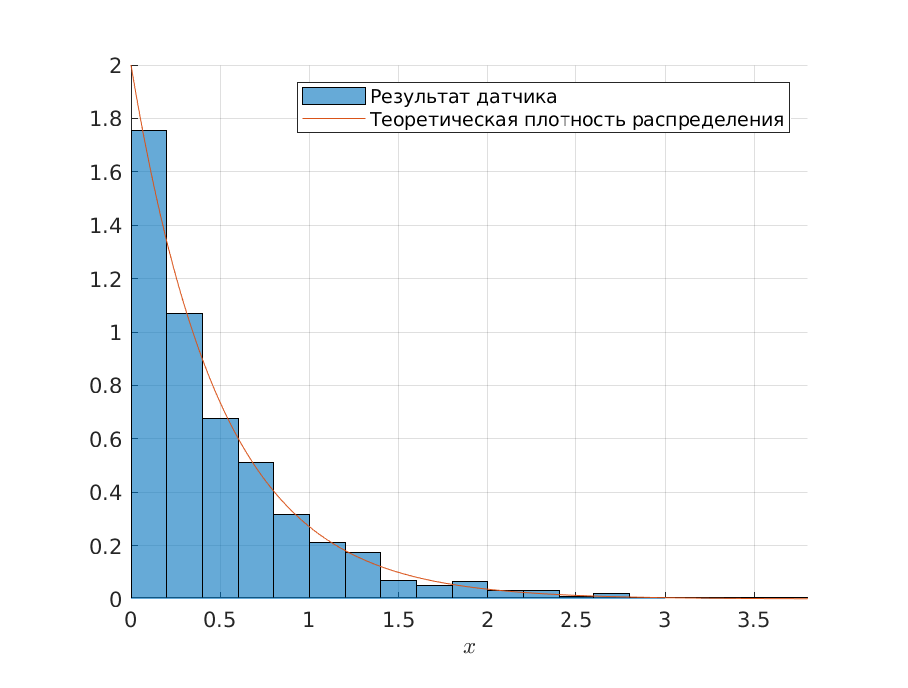
\includegraphics[width=0.5\linewidth]{task_03/exp2-1000.eps}
        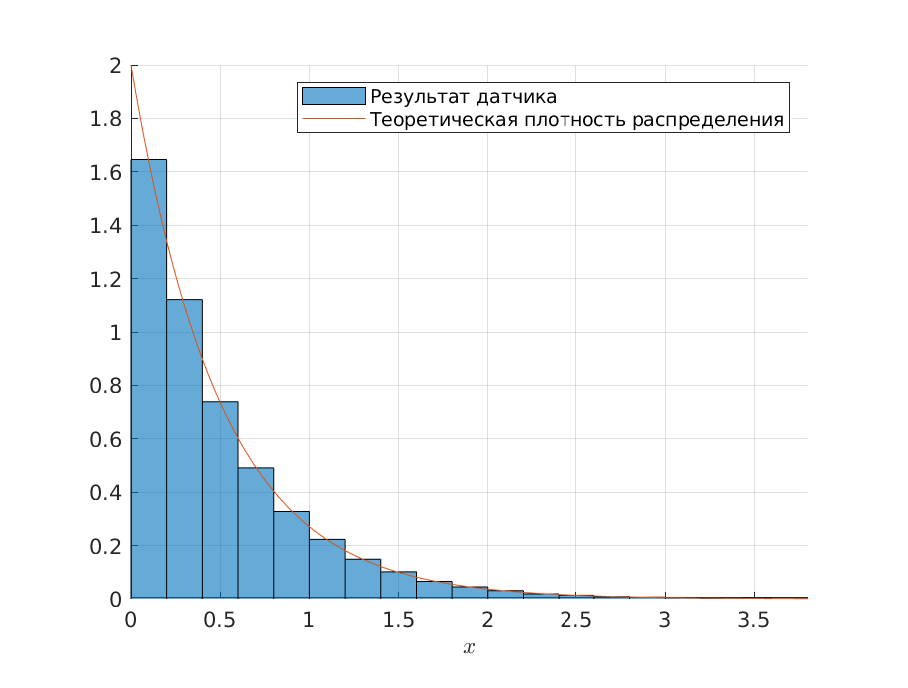
\includegraphics[width=0.5\linewidth]{task_03/exp2-100000.eps}
        \caption{Гистограмма экспоненциального распределения случайной величины с параметром $\lambda = 2$ при $10^3$~(слева) и $10^5$~(справа) испытаний.}
\end{figure}
\begin{figure}[h]
        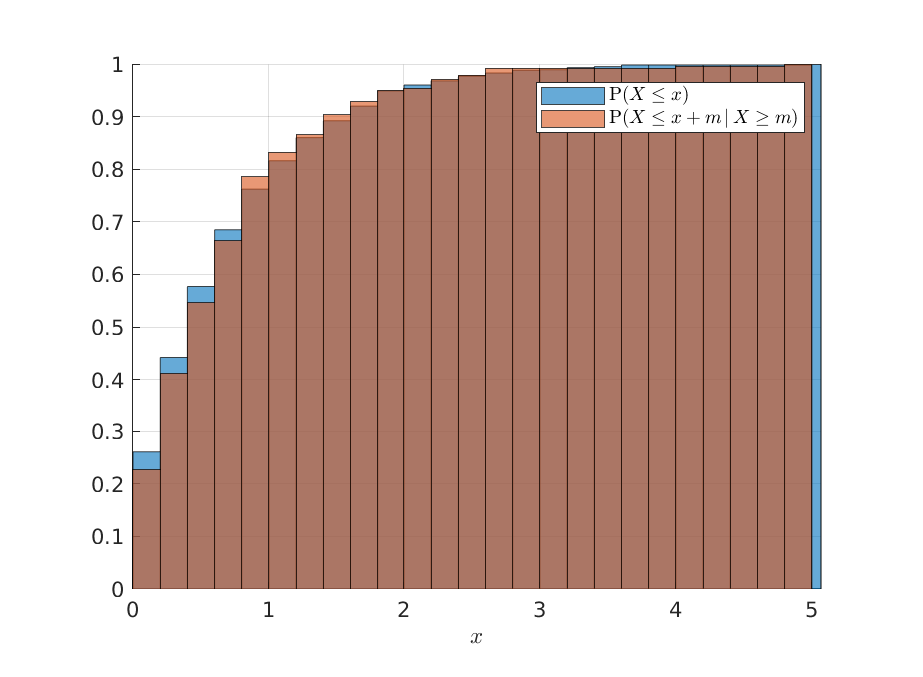
\includegraphics[width=\linewidth]{task_03/mem2-1000-1.eps}
        \caption{Гистограмма экспоненциального распределения, демонстрирующая его свойство отсутствия памяти. Здесь задан параметр распределения $\lambda = \frac{3}{2}$, а также <<сдвиг>> $m = 1$. Проведено $10^3$ испытаний.}
\end{figure}
\begin{figure}[h]
        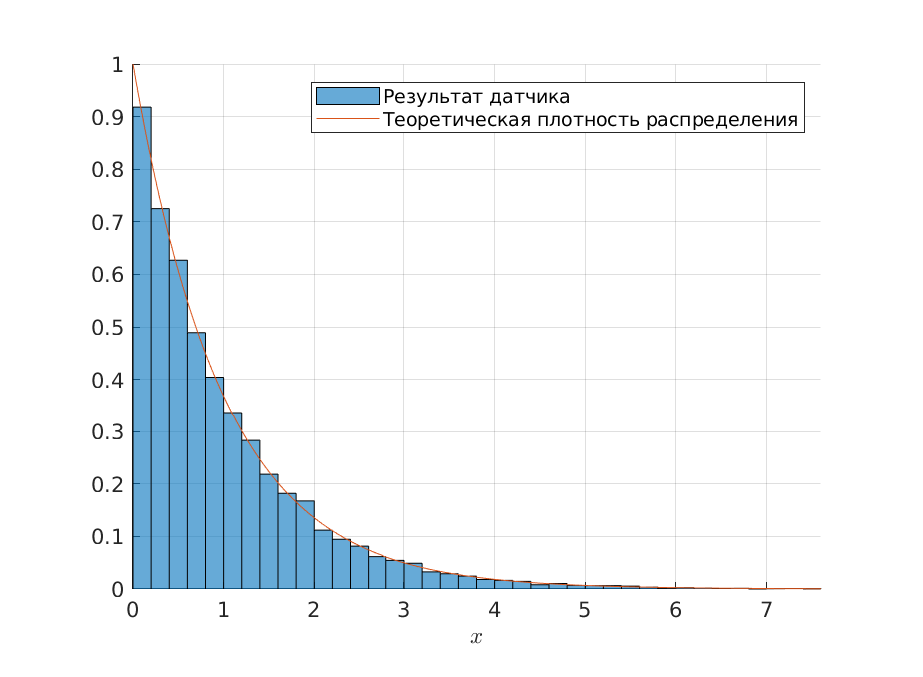
\includegraphics[width=\linewidth]{task_03/min-01-10-10000.eps}
        \caption{Гистограмма распределения случайной величины $Y = \min_{i = \overline{1, n}} X_i$. Здесь $\lambda_1 = \lambda_2 = \ldots = \lambda_n = \frac{1}{10}$, $n = 10$. Число испытаний $10^4$.}
\end{figure}
\begin{figure}[h]
        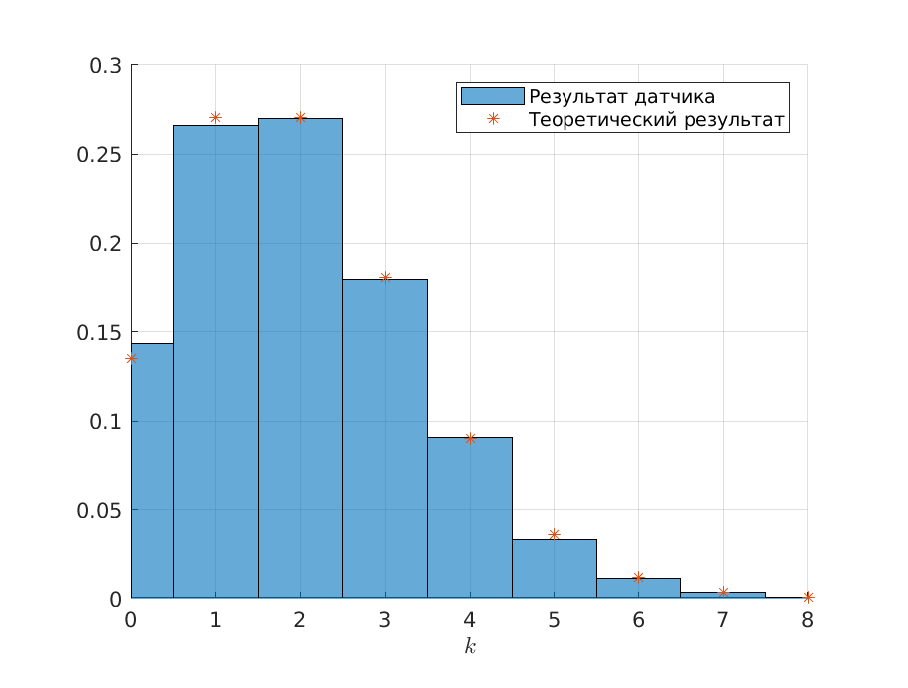
\includegraphics[width=0.5\linewidth]{task_03/pois2-10000.eps}
        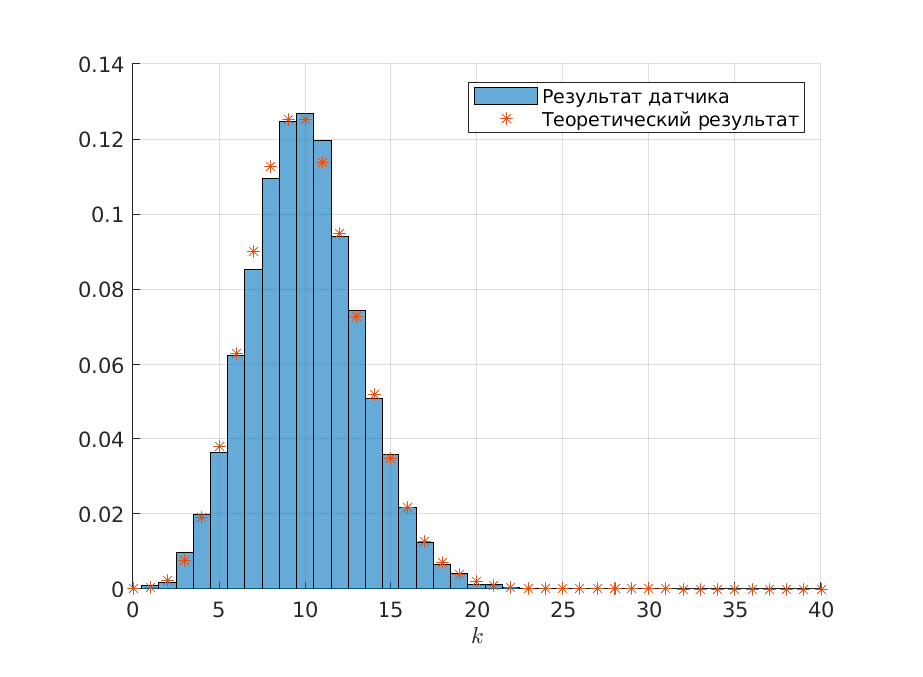
\includegraphics[width=0.5\linewidth]{task_03/pois10-10000.eps}
        \caption{Гистограмма распределения Пуассона случайной величины с параметром $\lambda = 2$~(слева) и $\lambda = 10$~(справа) при $10^4$~испытаний.}
\end{figure}